%\setcounter{section}{27}
\section{CÔNG THỨC CỘNG XÁC SUẤT}
\subsection{LÝ THUYẾT CẦN NHỚ}
\subsubsection{PHÉP TOÁN TRÊN CÁC BIẾN CỐ}
Cho hai biến cố $A$ và $B$. Khi đó $A, B$ là các tập con của không gian mẫu $\Omega$.
\begin{enumerate}[\iconMT]
	\immini{\item \indam{Biến cố hợp:} Biến cố: \lq\lq $A$ hoặc $B$ xảy ra\rq\rq\ được gọi là biến cố hợp của $A$ và $B$.
		\begin{itemize}
			\item  [$\bullet$] Kí hiệu là $A \cup B$.
			\item  [$\bullet$] Biến cố hợp $A \cup B$ là tập con của không gian mẫu $\Omega$.
		\end{itemize}
	}{
\begin{tikzpicture}[scale=1,rotate=5]
	\def\firstcircle{(0:0) ellipse (1.2 cm and 1 cm)}
	\def\secondcircle{(0:1.8) ellipse (1 cm and 1 cm)}
	\fill[pattern=north east lines] \firstcircle;
	\fill[pattern=north east lines] \secondcircle;
	\draw \firstcircle node[fill=white,left]{$A$};
	\draw \secondcircle node [fill=white,right=-0.1]{$B$};
\end{tikzpicture}}
	\immini{\item \indam{Biến cố giao:} Biến cố: \lq\lq Cả $A$ và $B$ đều xảy ra\rq\rq\ được gọi là biến cố giao của $A$ và $B$.
		\begin{itemize}
			\item [$\bullet$] Kí hiệu là $A \cap B$ hoặc $A B$;
			\item [$\bullet$] Biến cố giao $A \cap B$ là tập con  của không gian mẫu $\Omega$.
		\end{itemize}
	}{
\begin{tikzpicture}[scale=1,rotate=15]
	\def\firstcircle{(0:0) ellipse (1.2 cm and 1 cm)}
	\def\secondcircle{(0:1.5) ellipse (1 cm and 1 cm)}
	\begin{scope}
		\clip \secondcircle;
		\fill[pattern=north east lines] \firstcircle;
	\end{scope}
	\draw \firstcircle node[left]{$A$};
	\draw \secondcircle node [right]{$B$};
\end{tikzpicture}}
\immini{	\item \indam{Biến cố xung khắc:} Biến cố $A$ và biến cố $B$ được gọi là xung khắc nếu $A$ và $B$ không đồng thời xảy ra.
	Hai biến cố $A$ và $B$ xung khắc khi và chỉ khi $A \cap B=\varnothing$.
	\begin{luuy}
		Hai biến cố $A$ và $B$ là xung khắc khi và chỉ khi nếu biến cố này xảy ra thì biến cố kia không xảy ra.
	\end{luuy}}{
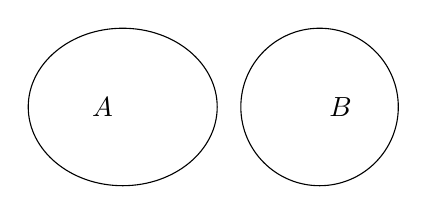
\begin{tikzpicture}[scale=1]
	\def\firstcircle{(0:0) ellipse (1.2 cm and 1 cm)}
	\def\secondcircle{(2.5,0) ellipse (1 cm and 1 cm)}
	\draw \firstcircle node[left]{$A$};
	\draw \secondcircle node [right]{$B$};
\end{tikzpicture}	}
\end{enumerate}

\subsubsection{CÔNG THỨC CỘNG XÁC SUẤT}


\begin{enumerate}[\iconMT]
	\item \indam{Công thức cộng xác suất:} Cho hai biến cố $A$ và $B$. Khi đó \boxmini{$\mathrm{P}(A \cup B) = \mathrm{P}(A) + \mathrm{P}(B) - \mathrm{P}(A \cap B)$}
	\item \indam{Đặt biệt:} Nếu hai biến cố $A$ và $B$ là xung khắc $\big(A \cap B = \varnothing\big)$ thì 
	\boxmini{$\mathrm{P}(A \cup B)=\mathrm{P}(A)+\mathrm{P}(B)$}
	\begin{luuy}
		Cho biến cố $A$ và biến cố đối $\overline{A}$. Ta có $\mathrm{P}(\overline{A})=1-\mathrm{P}(A)$.
	\end{luuy}
\end{enumerate}
\subsection{PHÂN LOẠI VÀ PHƯƠNG PHÁP GIẢI TOÁN}

\begin{dang}{Công thức cộng xác suất của hai biến cố xung khắc}
	\begin{enumerate}[\iconCH]
		\item Nếu hai biến cố $A$ và $B$ là xung khắc $\big(A \cap B = \varnothing\big)$ thì 
		\boxmini{$\mathrm{P}(A \cup B)=\mathrm{P}(A)+\mathrm{P}(B)$}
		\item Cho biến cố $A$ và $\overline{A}$ là biến cố đối của $A$. Khi đó, ta có 
		\boxmini{$\mathrm{P}(\overline{A})=1-\mathrm{P}(A)$}
	\end{enumerate}
\end{dang}

\begin{vd}%[1D2K2-5]
	Một hộp chứa $20$ tấm thẻ cùng loại được đánh số lần lượt từ $1$ đến $20$. Lấy ra ngẫu nhiên đồng thời $2$ thẻ từ hộp. Tính xác suất của các biến cố:
	\begin{enumerate}
		\item \lq\lq Tổng các số ghi trên $2$ thẻ lấy ra nhỏ hơn $4$ hoặc lớn hơn $37$\rq\rq;
		\item \lq\lq Tích các số ghi trên $2$ thẻ lấy ra chia hết cho $6$\rq\rq.
	\end{enumerate}
	\loigiai{
		\begin{enumerate}
			\item Gọi $A$ là biến cố \lq\lq Tổng các số ghi trên $2$ thẻ nhỏ hơn $4$\rq\rq. Biến cố $A$ xảy ra khi $2$ thẻ được chọn ghi số $1$ và $2$. Do đó $\mathrm{P}(A)=\dfrac{1}{\mathrm{C}_{20}^2}=\dfrac{1}{190}$.\\
			Gọi $B$ là biến cố \lq\lq Tổng các số ghi trên $2$ thẻ lớn hơn $37$\rq\rq. Biến cố $B$ xảy ra khi $2$ thẻ được chọn ghi số $20$ và $18$ hoặc $20$ và $19$. Do đó $\mathrm{P}(B)=\dfrac{2}{\mathrm{C}_{20}^2}=\dfrac{2}{190}$.\\
			Do $A$ và $B$ là hai biến cố xung khắc nên xác suất của biến cố \lq\lq Tổng các số ghi trên $2$ thẻ lấy ra nhỏ hơn $4$ hoặc lớn hơn $37$\rq\rq~là
			$$
			\mathrm{P}(A \cup B)=\mathrm{P}(A)+P(B)=\dfrac{3}{190}.
			$$
			\item Gọi $D$ là biến cố \lq\lq Trong $2$ thẻ lấy ra có ít nhất $1$ thẻ ghi số chia hết cho $6$\rq\rq.\\
			Do có $3$ thẻ chia hết cho $6$ nên xác suất của biến cố \lq\lq Trong $2$ thẻ lấy ra không có thẻ nào ghi số chia hết cho $6$\rq\rq~là
			$$
			\mathrm{P}\left(\overline{D}\right)=\dfrac{\mathrm{C}_{17}^2}{\mathrm{C}_{20}^2}=\dfrac{68}{95}.
			$$		
			Vậy xác suất của biến cố $D$ là
			$$
			\mathrm{P}(D)=1-\mathrm{P}\left(\overline{D}\right)=\dfrac{27}{95}.
			$$
			Gọi $E$ là biến cố \lq\lq Tích các số ghi trên $2$ thẻ lấy ra chia hết cho 6 nhưng không có thẻ nào ghi số chia hết cho $6$\rq\rq. Biến cố $E$ xảy ra khi trong hai thẻ lấy ra có một thẻ ghi số chẵn nhưng không chia hết cho $3$ (có $7$ thẻ như vậy) và thẻ còn lại ghi số chia hết cho $3$ nhưng không chia hết cho $6$ (có $3$ thẻ như vậy).\\		
			Vậy xác suất của biến cố $E$ là
			$$
			\mathrm{P}(E)=\dfrac{7\cdot 3}{\mathrm{C}_{20}^2}=\dfrac{21}{190}.
			$$		
			Do $D$ và $E$ là hai biến cố xung khắc nên xác suất của biến cố \lq\lq Tích các số ghi trên $2$ thẻ lấy ra chia hết cho $6$\rq\rq~là
			$$
			\mathrm{P}(D \cup E)=\mathrm{P}(D)+\mathrm{P}(E)=\dfrac{15}{38}.
			$$
		\end{enumerate}
	}
\end{vd}
\dongcham{11}
\begin{vd}%[1D2B2-5]
	Một hộp chứa $4$ viên bi xanh, $5$ viên bi đỏ và $3$ viên bi vàng có cùng kích thước và khối lượng. Chọn ra ngẫu nhiên $4$ viên bi từ hộp. Tính xác suất của các biến cố:
	\begin{enumerate}
		\item \lq\lq Cả 4 viên bi lấy ra đều có cùng màu\rq\rq;
		\item \lq\lq Có ít nhất 3 viên bi xanh trong 4 viên bi lấy ra\rq\rq.
	\end{enumerate}
	\loigiai{
		\begin{enumerate}
			\item Gọi $A$ là biến cố \lq\lq Cả 4 viên bi lấy ra đều có cùng màu xanh\rq\rq, $B$ là biến cố \lq\lq Cả $4$ viên bi lấy ra có cùng màu đỏ\rq\rq. Vì chỉ có $3$ viên bi màu vàng nên $A \cup B$ là biến cố \lq\lq Cả $4$ viên bi lấy ra có cùng màu\rq\rq. Do $A$ và $B$ là hai biến cố xung khắc nên
			$$
			\mathrm{P}(A \cup B)=\mathrm{P}(A)+\mathrm{P}(B)=\dfrac{\mathrm{C}_4^4}{\mathrm{C}_{12}^4}+\dfrac{\mathrm{C}_5^4}{\mathrm{C}_{12}^4}=\dfrac{2}{165} .
			$$
			\item Gọi $C$ là biến cố \lq\lq Có $3$ viên bi xanh trong $4$ viên lấy ra\rq\rq. Khi đó $A \cup C$ là biến cố \lq\lq Có ít nhất $3$ viên bi xanh trong $4$ viên bi lấy ra\rq\rq. Do $A$ và $C$ là hai biến cố xung khắc nên
			$$
			\mathrm{P}(A \cup C)=\mathrm{P}(A)+\mathrm{P}(C)=\dfrac{\mathrm{C}_4^4}{\mathrm{C}_{12}^4}+\dfrac{\mathrm{C}_4^3 \mathrm{C}_8^1}{\mathrm{C}_{12}^4}=\dfrac{1}{15}.
			$$
		\end{enumerate}
	}
\end{vd}\dongcham{9}

\begin{vd}%[1D2B2-6]
	Trong một căn phòng có $36$ người, trong đó có $25$ người họ Nguyễn và $11$ người họ Trần. Chọn ngẫu nhiên hai người trong phòng đó. Tính xác suất để hai người được chọn có cùng họ.
	\loigiai{
		Gọi $A$ là biến cố: \lq\lq Cả hai người được chọn đều họ Nguyễn\rq\rq, $B$ là biến cố: \lq\lq Cả hai người được chọn đều họ Trần\rq\rq.\\
		$C$ là biến cố: \lq\lq Cả hai người được chọn có cùng họ\rq\rq. $C$ là biến cố hợp của $A$ và $B$. Do $A$ và $B$ xung khắc nên  
		$$\mathrm{P}(C)=\mathrm{P}(A \cup B)=\mathrm{P}(A)+\mathrm{P}(B).$$
		Ta có: $n(\Omega)=\mathrm{C}_{36}^{2}=630; n(A)=\mathrm{C}_{25}^{2}=300; n(B)=\mathrm{C}_{11}^{2}=55.$ Khi đó
		$$\mathrm{P}(A)=\dfrac{n(A)}{n(\Omega)} = \dfrac{300}{630}; \mathrm{P}(B)=\dfrac{n(B)}{n(\Omega)} = \dfrac{55}{630}.$$
		Vậy $\mathrm{P}(C)=\mathrm{P}(A)+\mathrm{P}(B)=\dfrac{300}{630}+\dfrac{55}{630}=\dfrac{355}{630}=\dfrac{71}{126}.$
	}	
\end{vd}\dongcham{8}

\begin{vd}%[1D2K2-3]
	Một hộp chứa 10 quả bóng xanh và 10 quả bóng đỏ có kích thước và khối lượng như nhau. Lấy ra ngẫu nhiên đồng thời 5 quả bóng từ hộp. Tính xác suất của biến cố \text{\lq\lq} có ít nhất 3 quả bóng xanh trong 5 quả bóng lấy ra\text{\rq\rq}.
	\loigiai{
		Ta có sơ đồ sau:
		\begin{center}
			\begin{tikzpicture}[line join = round, line cap = round,>=stealth,font=\footnotesize,scale=1]
				\def \goc{70}
				\def \r{1.5}
				\pgfmathsetmacro{\ngang}{\r/cos(\goc)}
				\coordinate (O) at (0,0);
				\draw (O)--++(-90:\r) node[below]{$\begin{matrix}
						4\text{ bóng xanh}\\
						1\text{ bóng đỏ}\\
						\mathrm{C}_{10}^{4}\cdot\mathrm{C}_{10}^{1}
					\end{matrix}$}	;
				\draw (O)--++({-90+\goc}:\ngang) node[below]{$\begin{matrix}
						5\text{ bóng xanh}\\
						\\
						\mathrm{C}_{10}^{5}
					\end{matrix}$};
				\draw (O)--++({-90-\goc}:\ngang) node[below]{$\begin{matrix}
						3\text{ bóng xanh}\\
						2\text{ bóng đỏ}\\
						\mathrm{C}_{10}^{3}\cdot\mathrm{C}_{10}^{2}
					\end{matrix}$};
			\end{tikzpicture}
		\end{center}
		\begin{itemize}
			\item [$\bullet$] Trường hợp lấy được  3 quả bóng xanh và 2 quả bóng đỏ, ta tính được xác xuất là $$P(A)=\dfrac{\mathrm{C}_{10}^3\mathrm{C}_{10}^2}{\mathrm{C}_{20}^5}$$
			\item [$\bullet$] Trường hợp lấy được  4 quả bóng xanh và 1 quả bóng đỏ, ta tính được xác xuất là $$P(B)=\dfrac{\mathrm{C}_{10}^4\mathrm{C}_{10}^1}{\mathrm{C}_{20}^5}$$
			\item [$\bullet$] Trường hợp lấy được  5 quả bóng xanh và 0 quả bóng đỏ, ta tính được xác xuất là $$P(C)=\dfrac{\mathrm{C}_{10}^5\mathrm{C}_{10}^0}{\mathrm{C}_{20}^5}$$
		\end{itemize}
		Xác suất của biến cố \text{\lq\lq}Có ít nhất $3$ quả bóng xanh trong $5$ quả bóng lấy ra\text{\rq\rq} là $$P(A)+P(B)+P(C)=\dfrac 12$$
	}
\end{vd}\dongcham{10}

\begin{vd}
	Một lớp có $41$ học sinh trong đó có $15$ bạn nam và $26$ bạn nữ. Cô giáo chủ nhiệm chọn ngẫu nhiên ra bốn bạn đi trực ban. 
	\begin{tasks}(1)
		\task Tính xác suất để cả bốn bạn đó đều là nữ.
		\task Tính xác suất để có ít nhất một bạn nam.
	\end{tasks}
	\loigiai{
		Ta có $n(\Omega)=C_{41}^4$.
		\begin{enumerate}[a)]
			\item Gọi $A$ là biến cố: \lq\lq Cả bốn bạn đều là nữ\rq\rq.\\
			$n(A)=C_{26}^4$.\\
			Vậy $\mathrm{P}(A)=\dfrac{C_{26}^4}{C_{41}^4}=\dfrac{115}{779}$.
			\item Gọi $B$ là biến cố: \rq\rq Có ít nhất một bạn nam\rq\rq.\\
			Ta có $B=\overline{A}$. Do đó $\mathrm{P}(B)=1-\mathrm{P}(A)=\dfrac{664}{779}$.
		\end{enumerate}
	}
\end{vd}\dongcham{12}

\begin{vd}
	Có hai hòm đựng thẻ, mỗi hòm đựng $10$ thẻ đánh số từ $1$ đến $10$. Lấy ngẫu nhiên từ mỗi hòm một thẻ. Tính xác suất để trong hai thẻ lấy ra
	\begin{tasks}(2)
		\task có ít nhất một thẻ đánh số $1$.
		\task tổng hai số ghi trên hai thẻ khác $19$.
	\end{tasks}
	\loigiai{
		Ta có $n(\Omega)=C_{10}^1.C_{10}^1$.
		\begin{enumerate}[a)]
			\item Gọi $A$ là biến cố: \lq\lq Lấy được ít nhất một thẻ đánh số $1$\rq\rq.\\
			Khi đó, $\overline{A}$ là biến cố: \lq\lq Cả hai thẻ đều không đánh số $1$\rq\rq.\\
			Ta có $n\left(\overline{A}\right)=C_9^1.C_9^1\Rightarrow \mathrm{P}\left(\overline{A}\right)=\dfrac{C_9^1.C_9^1}{C_{10}^1.C_{10}^1}$.\\
			Vậy $\mathrm{P}(A)=1-\mathrm{P}\left(\overline{A}\right)=\dfrac{19}{100}$.
			\item Gọi $B$ là biến cố: \lq\lq Tổng hai số ghi trên thẻ khác $19$\rq\rq.\\
			Khi đó, $\overline{B}$ là biến cố: \lq\lq Tổng hai số ghi trên thẻ bằng $19$\rq\rq.\\
			Ta có $n\left(\overline{B}\right)=2\Rightarrow \mathrm{P}(B)=\dfrac{2}{C_{10}^1.C_{10}^1}$.\\
			Vậy $\mathrm{P}(B)=1-\mathrm{P}\left(\overline{B}\right)=\dfrac{49}{50}$.
		\end{enumerate}
	}
\end{vd}\dongcham{12}

\begin{dang}{Công thức cộng xác suất của hai biến cố bất kì}
	Cho hai biến cố $A$ và $B$. Khi đó \boxmini{$\mathrm{P}(A \cup B) = \mathrm{P}(A) + \mathrm{P}(B) - \mathrm{P}(A \cap B)$}
\end{dang}
\begin{vd}%[1D2B2-6]
	Tung một đồng xu cân đối và đồng chất hai lần liên tiếp.
	\begin{enumerate}
		\item Viết các kết quả thuận lợi của không gian mẫu $\Omega$ và hai biến cố
		\begin{enumerate}[]
			\item $A\colon$``Có ít nhất một lần xuất hiện mặt sấp'';
			\item $B\colon$``Có ít nhất một lần xuất hiện mặt ngửa''.
		\end{enumerate}
		\item Viết các kết quả thuận lợi của mỗi biến cố $A\cup B$, $A \cap B$.
		\item Tính $P(A), P(B),P(A\cup B), P(A\cap B)$.
	\end{enumerate}
	\loigiai{
		\begin{enumerate}
			\item Kí hiệu $S$ là mặt sấp, $N$ là mặt ngửa. Ta có
			$$\Omega=\{ SS;SN;NS;NN \} ; A=\{ SS;SN;NS \} ; B=\{ SN;NS;NN \}.$$
			\item Ta có
			$$A\cup B=\{ SS;SN;NS;NN \} =\Omega; A \cap B=\{ SN;NS \}.$$
			\item Ta có 
			\begin{enumerate}[]
				\item $P(A)=\dfrac{n(A)}{n(\Omega)}=\dfrac{3}{4}$; $P(B)=\dfrac{n(B)}{n(\Omega)}=\dfrac{3}{4}$.
				\item $P(A\cup B)=\dfrac{n(A\cup B)}{n(\Omega)}=1$;
				$P(A\cap B)=\dfrac{n(A\cap B)}{n(\Omega)}=\dfrac{1}{2}$.
			\end{enumerate}
		\end{enumerate}
	}	
\end{vd}\dongcham{14}

\begin{vd}%[1K8BR-2]
	Một hộp đựng $25$ tấm thẻ cùng loại được đánh số từ $1$ đến $25$. Rút ngẫu nhiên một tấm thẻ trong hộp. Xét các biến cố $P$ : \lq\lq Số ghi trên tấm thẻ là số chia hết cho $4$\rq\rq; $Q$: \lq\lq Số ghi trên tấm thẻ là số chia hết cho $6$\rq\rq.
	\begin{enumerate}
		\item Mô tả không gian mẫu.
		\item Xác định các biến cố $P$, $Q$ và  $S=P\cap Q$.
		\item Tính xác suất của biến cố $P \cup Q$.
	\end{enumerate} 
	\loigiai{
		\begin{enumerate}
			\item $\Omega=\{1,2,3,4,5,6,7,8,9,10,11,12,13,14,15,16,17,18,19,20,21,22,23,24,25\}$.
			\item 	Ta có: $P=\{4,8,12,16,20,24\}$; $Q=\{6,12,18,24\}$.\\
			$S=P \cap Q=\{12;24\}$ là biến cố \lq\lq Số ghi trên tấm thẻ là số chia hết cho $4$ và chia hết cho $6$\rq\rq.
			\item Ta có $\mathrm{P}(P \cup Q) = \mathrm{P}(P) + \mathrm{P}(Q) - \mathrm{P}(P \cap Q)=\dfrac{6}{25}+\dfrac{4}{25}-\dfrac{2}{25}=\dfrac{8}{25}$.
		\end{enumerate} 
	}
\end{vd}\dongcham{9}

\begin{vd}
	Lớp 11A có $44$ học sinh trong đó có $14$ học sinh đạt điểm tổng kết môn Hóa học loại giỏi và $15$ học sinh đạt điểm tổng kết môn Vật lý loại giỏi. Biết rằng khi chọn một học sinh của lớp đạt điểm tổng kết môn Hóa học hoặc Vật lý loại giỏi có xác suất là $0{,}5$. Số học sinh đạt điểm tổng kết giỏi cả hai môn Hóa học và Vật lý là
	\loigiai{
		Đặt $A$ là biến cố học sinh đạt điểm tổng kết môn Hóa học loại giỏi.\\
		$B$ là biến cố học sinh đạt điểm tổng kết môn Vậy lý loại giỏi.\\
		Ta có $A\cap B$ là biến cố học sinh đạt điểm tổng kết môn Hóa học và Vật lý loại giỏi.\\
		$A\cup B$ là biến cố học sinh đạt điểm tổng kết môn Hóa học hoặc Vật lý loại giỏi.\\
		Khi đó $\mathrm{P}(A\cap B)=\mathrm{P}(A)+\mathrm{P}(B)-\mathrm{P}(A\cup B)=\dfrac{14}{44}+\dfrac{15}{44}-0{,}5=\dfrac{7}{44}$.\\
		Do đó số học sinh đạt điểm tổng kết giỏi cả hai môn Hóa học và Vật lý là $7$ học sinh.
	}
\end{vd}\dongcham{9}

\begin{vd}%[1D2K2-5]
	Gieo ngẫu nhiên 3 con xúc xắc cân đối và đồng chất. Tính xác suất của biến cố 
	$A$: \text{\lq\lq}Tích số chấm xuất hiện trên mỗi con xúc xắc chia hết cho 15\text{\rq\rq}.
	\loigiai
	{
		Gọi $B$ là biến cố \text{\lq\lq}Tích số chấm xuất hiện trên mỗi con xúc xắc không chia hết cho 5\text{\rq\rq}, $C$ là biến cố \text{\lq\lq}Tích số chấm xuất hiện trên mỗi con xúc xắc không chia hết cho 3\text{\rq\rq}.\\
		Khi đó, $A$ là biến cố đối của biến cố $B\cup C$.\\
		Ta có $\mathrm{P}(B\cup C)=\mathrm{P}(B)+\mathrm{P}(C)-\mathrm{P}(B\cap C)=\left(\dfrac{5}{6}\right)^3+\left(\dfrac{4}{6}\right)^3-\left(\dfrac{3}{6}\right)^3=\dfrac{3}{4}$.\\
		Do đó, xác suất của biến cố $A$: \text{\lq\lq}Tích số chấm xuất hiện trên mỗi con xúc xắc chia hết cho 15\text{\rq\rq} là 
		\[\mathrm{P}(A)=1-\mathrm{P}(B \cup C)=1-\dfrac{3}{4}=\dfrac{1}{4}.\]
	}
\end{vd}\dongcham{10}

\begin{vd}%[1D2K2-6]
	Trong một công ty có $40$ nhân viên, trong đó có $19$ người thích chơi bóng bàn, $20$ người thích chơi cầu lông, $8$ người không thích chơi cả cầu lông và bóng bàn. Chọn ngẫu nhiên một nhân viên trong công ty đó. Tính xác suất để người đó
	\begin{enumerate}
		\item Thích chơi ít nhất một trong hai môn bóng bàn và cầu lông.
		\item Thích chơi cầu lông và không thích chơi bóng bàn.
		\item Thích chơi bóng bàn và không thích chơi cầu lông.
		\item Thích chơi đúng một trong hai môn.
	\end{enumerate}
	\loigiai{
		Gọi $A$ là biến cố: \lq\lq Người đó thích chơi bóng bàn\rq\rq, $B$ là biến cố: \lq\lq Người đó thích chơi cầu lông\rq\rq.
		\begin{enumerate}
			\item Biến cố đối của biến cố $A \cup B$: \lq\lq Người đó thích chơi ít nhất một trong hai môn\rq\rq là biến cố $\overline{AB}$: \lq\lq Người đó không thích chơi ít nhất một trong hai môn\rq\rq.\\
			Ta có: $\mathrm{P}(A) = \dfrac{19}{40}; \mathrm{P}(B)=\dfrac{20}{40}; \mathrm{P}(\overline{AB})=\dfrac{8}{40}.$\\
			Vậy $\mathrm{P}(A \cup B)=1-\mathrm{P}(\overline{AB})=1-\dfrac{8}{40}=\dfrac{32}{40}=\dfrac{4}{5}.$
			\item Ta có: $\mathrm{P}(A B)=\mathrm{P}(A)+\mathrm{P}(B)-\mathrm{P}(A \cup B)=\dfrac{19}{40}+\dfrac{20}{40}-\dfrac{32}{40}=\dfrac{7}{40}.$\\
			$B=AB \cup \overline{A}B$, suy ra $\mathrm{P}(B )=\mathrm{P}(AB)+\mathrm{P}(\overline{A}B)$.\\ Vậy $\mathrm{P}(\overline{A}B)=\mathrm{P}(B )-\mathrm{P}(AB)=\dfrac{20}{40}-\dfrac{7}{40}=\dfrac{13}{40}.$
			\item Ta có: $A=AB \cup A\overline{B}$, suy ra $\mathrm{P}(A )=\mathrm{P}(AB)+\mathrm{P}(A\overline{B})$.\\
			Vậy $\mathrm{P}(A\overline{B})=\mathrm{P}(A )-\mathrm{P}(AB)=\dfrac{19}{40}-\dfrac{7}{40}=\dfrac{12}{40}=\dfrac{3}{10}.$
			\item Gọi $E$ là biến cố: \lq\lq Người đó thích chơi đúng một trong hai môn cầu lông hay bóng bàn\rq\rq.\\
			Ta có: $E=A\overline{B} \cup \overline{A}B$, suy ra $\mathrm{P}(E)=A\overline{B}+\overline{A}B=\dfrac{12}{40}+\dfrac{13}{40}=\dfrac{25}{40}=\dfrac{5}{8}.$
		\end{enumerate}
	}	
\end{vd}
\dongcham{26}
\subsection{BÀI TẬP TỰ LUYỆN}

\begin{baitap}
	Gieo hai con xúc xắc cân đối và đồng chất. Gọi $A$ là biến cố \lq\lq Tổng số chấm xuất hiện trên hai con xúc xắc bằng 5\rq\rq, $B$ là biến cố \lq\lq Tích số chấm xuất hiện trên hai con xúc xắc bằng 6\rq\rq.
	\begin{enumerate}
		\item Hãy viết tập hợp mô tả các biến cố trên.
		\item Hãy liệt kê các kết quả của phép thử làm cho cả hai biến cố $A$ và $B$ cùng xảy ra.
	\end{enumerate}
	\loigiai{
		\begin{enumerate}
			\item 	Biến cố $A=\{(1 ; 4) ;(4 ; 1) ;(2 ; 3) ;(3 ; 2)\}$.\\
			Biến cố $B=\{(1 ; 6) ;(6 ; 1) ;(2 ; 3) ;(3 ; 2)\}$.
			\item Kết quả của phép thử làm cho cả hai biến cố $A$ và $B$ cùng xảy ra là $\{(2 ; 3) ;(3 ; 2)\}$.
		\end{enumerate}
	}
\end{baitap}

\begin{baitap}%[1D2B1-3]
	Tung một đồng xu cân đối và đồng chất ba lần liên tiếp. Xét các biến cố:
	\begin{enumerate}[]
		\item $A$: ``Đồng xu xuất hiện mặt sấp (S) ở lần tung thứ nhất''.
		\item $B$: ``Đồng xu xuất hiện mặt ngửa (N) ở lần tung thứ nhất''.
	\end{enumerate}
	Hai biến cố trên có xung khắc hay không? Vì sao?
	\loigiai{
		Ta có $\begin{aligned}[t]
			A&=\{\text{SSS;SSN;SNS;SNN}\}\\
			B&=\{\text{NSS;NSN;NNS;NNN}\}.
		\end{aligned}$\\
		Suy ra $A \cap B=\varnothing$. Do đó $A$ và $B$ là hai biến cố xung khắc.
	}
\end{baitap} 

\begin{baitap}%[1D2Y1-1]
	Hai xạ thủ $X$, $Y$ mỗi người bắn một viên đạn vào một mục tiêu. Xét các biến cố $A$: \lq\lq Xạ thủ $X$ bắn trúng\rq\rq; $B$: \lq\lq Xạ thủ $Y$ bắn trúng\rq\rq. Nêu nội dung của các biến cố $AB$, $A \cup B$, $\overline{AB}$, $\overline{A}B$, $A\overline{B}$, $\overline{A}B \cup A\overline{B}$.
	\loigiai{
		\begin{itemize}
			\item $AB$: \lq\lq Cả hai xạ thủ bắn trúng \rq\rq.
			\item $A \cup B$: \lq\lq Có ít nhất một xạ thủ bắn trúng \rq\rq.
			\item $\overline{AB}$: \lq\lq Cả hai xạ thủ bắn trượt \rq\rq.
			\item $\overline{A}B$: \lq\lq Xạ thủ $X$ bắn trượt, xạ thủ $Y$ bắn trúng \rq\rq.
			\item $A\overline{B}$: \lq\lq Xạ thủ $X$ bắn trúng, xạ thủ $Y$ bắn trượt \rq\rq.
			\item $\overline{A}B \cup A\overline{B}$: \lq\lq Chỉ có một xạ thủ bắn trúng \rq\rq.
		\end{itemize}
	}
\end{baitap}

\begin{baitap}%[1D2Y2-6]
	Trong một hộp có 8 viên bi xanh và 6 viên bi đỏ. Lấy ngẫu nhiên 2 viên bi trong hộp. Gọi $A$ là biến cố: \lq\lq Cả hai viên bi có màu xanh\rq\rq; $B$ là biến cố: \lq\lq có một viên bi màu xanh và một viên bi màu đỏ\rq\rq.
	\begin{enumerate}
		\item Tính $\mathrm{P}(A)$ và $\mathrm{P}(B).$
		\item Tính xác suất để trong hai viên bi lấy ra có ít nhất một viên bi màu xanh.
	\end{enumerate}
	\loigiai{
		\begin{enumerate}
			\item Ta có $n(\Omega)=\mathrm{C}^2_{14}= 91$; $n(A)=\mathrm{C}^2_{8}= 28$, $n(B)=8\cdot 6= 48$.\\
			Vậy $\mathrm{P}(A)=\dfrac{n(A)}{n(\Omega)} = \dfrac{28}{91}$, $\mathrm{P}(B)=\dfrac{n(B)}{n(\Omega)} = \dfrac{48}{91}$.
			\item \textbf{Cách 1:} Xét biến cố $C$: \lq\lq Trong hai viên bi lấy ra có ít nhất một viên bi màu xanh \rq\rq, nên $C$ là biến cố hợp của $A$ và $B$. Do $A$ và $B$ là hai biến cố xung khắc nên $\mathrm{P}(C)=\mathrm{P}(A)+\mathrm{P}(B)= \dfrac{28}{91}+\dfrac{48}{91}=\dfrac{76}{91}.$\\
			\textbf{Cách 2:} Xét biến cố đối $\overline{C}$: \lq\lq Cả hai viên bi lấy ra đều có màu đỏ \rq\rq. Khi đó $n(\overline{C})=\mathrm{C}^2_{6}= 15$. Suy ra $\mathrm{P}(\overline{C})=\dfrac{15}{91}$. \\
			Vậy $\mathrm{P}(C)=1-\mathrm{P}(\overline{C})= 1-\dfrac{15}{91}=\dfrac{76}{91}.$
		\end{enumerate}
	}
\end{baitap} \cham{10}
\begin{baitap}
	Trong bình đựng có 10 viên bi, trong đó có 4 viên bi đỏ. Lấy ngẫu nhiên 3 viên bi. Tính xác suất để trong 3 viên bi lấy được 1 hoặc 2 viên bi đỏ.
	\loigiai{
		Đặt $A_1$ là biến cố ``trong 3 viên lấy ra được đúng 1 viên bi đỏ'' và $A_2$ là biến cố ``trong 3 viên lấy ra có đúng 2 viên bi đỏ''.\\
		Ta phải tính xác suất của biến cố $A$ là biến cố trong 3 viên lấy ra một hoặc hai viên bi đỏ. Các biến cố $A_1$ và $A_2$ là xung khắc. Do đó
		\[\mathrm{P}(A_1 + A_2) = \mathrm{P}(A_1) + \mathrm{P}(A_2)\]
		\[\mathrm{P}(A_1) = \frac{\mathrm{C_{4}^1} \mathrm{C_{6}^2}}{\mathrm{C_{10}^3}} = \frac{1}{2}\]
		\[\mathrm{P}(A_2) = \frac{\mathrm{C_{4}^2} \mathrm{C_{6}^1}}{\mathrm{C_{10}^3}} = \frac{3}{10}\]
		Vậy
		\[\mathrm{P}(A) = \frac{1}{2} + \frac{3}{10} = \frac{4}{5}.\]
	}
\end{baitap} \cham{11}


\begin{baitap}%[1D2K2-5]
	Một hộp chứa 40 tấm thẻ cùng loại được đánh số lần lượt từ 1 đến 40. Lấy ra ngẫu nhiên đồng thời hai thẻ từ hộp. Tính xác suất của các biến cố:
	\begin{enumerate}
		\item \text{\lq\lq}Tổng các số ghi trên 2 thẻ lấy ra nhỏ hơn 4 hoặc lớn hơn 76\text{\rq\rq}.
		\item \text{\lq\lq}Tích các số ghi trên 2 thẻ lấy ra chia hết cho 10\text{\rq\rq}.
	\end{enumerate}
	\loigiai
	{
		\begin{enumerate}
			\item Gọi $A$ là biến cố \text{\lq\lq}Tổng các số ghi trên 2 thẻ lấy ra nhỏ hơn 4 hoặc lớn hơn 76\text{\rq\rq}. Gọi $A_1$ là biến cố \text{\lq\lq}Tổng các số ghi trên 2 thẻ lấy ra nhỏ hơn 4\text{\rq\rq}, $A_2$ là biến cố \text{\lq\lq}Tổng các số ghi trên 2 thẻ lấy ra lớn hơn 76\text{\rq\rq}.\\
			Khi đó, ta có $A=A_1\cup A_2$.\\
			Biến cố $A_1$ xảy ra khi 2 tấm thẻ được chọn ghi số 1 và 2. Do đó $\mathrm{P}(A_1)=\dfrac{1}{\mathrm{C}_{40}^2}$.\\
			Biến cố $A_2$ xảy ra khi 2 tấm thẻ được chọn ghi số $(37;40),(38;40),(39;40)$ hoặc $(38;39)$. Do đó, $\mathrm{P}(A_2)=\dfrac{4}{\mathrm{C}_{40}^2}$.\\
			Do $A_1$ và $A_2$ là hai biến cố xung khắc nên:
			\[\mathrm{P}(A)=P\left(A_1 \cup A_2\right)=\mathrm{P}(A_1)+\mathrm{P}(A_2)=\dfrac{1}{156}.\]
			\item Từ 1 đến 40 có 8 số chia hết cho $5;20$ số chia hết cho 2 và 4 số chia hết cho 10. Gọi $B$ là biến cố\text{\lq\lq}Tích các số ghi trên 2 thẻ lấy ra chia hết cho 10\text{\rq\rq}.\\
			Gọi $B_1$ là biến cố\text{\lq\lq}Tích các số ghi trên 2 thẻ lấy ra không chia hết cho 5\text{\rq\rq}, $B_2$ là biến cố\text{\lq\lq}Tích các số ghi trên 2 thẻ lấy ra không chia hết cho 2\text{\rq\rq}.\\
			Khi đó, $B$ là biến cố đối của biến cố $B_1\cup B_2$.\\
			Ta có 
			\[P\left(B_1 \cup B_2\right)=\mathrm{P}(B_1)+\mathrm{P}(B_2)-\mathrm{P}(B_1 B_2)=\dfrac{ \mathrm{C}_{32}^2}{ \mathrm{C}_{40}^2}+\frac{ \mathrm{C}_{20}^2}{ \mathrm{C}_{40}^2}-\frac{ \mathrm{C}_{16}^2}{ \mathrm{C}_{40}^2}=\dfrac{283}{390}.\]
			Do đó, xác suất biến cố $B$ \text{\lq\lq}Tích các số ghi trên hai thẻ chia hết cho 10\text{\rq\rq} là 
			\[\mathrm{P}(B)=1-P\left(B_1 \cup B_2\right)=\dfrac{107}{390}.\]
			
		\end{enumerate}
	}
\end{baitap} \cham{10}

\begin{baitap}%[Vũ Hồng Toàn]%[1D2K2-6]%BT22
	Một lớp có $40$ học sinh, trong đó có $34$ em thích ăn chuối, $22$ em thích ăn cam và $2$ em không thích ăn cả hai loại quả đó. Chọn ngẫu nhiên một học sinh trong lớp. Tính xác suất để em đó:
	\begin{enumerate}[a)]
		\item Thích ăn ít nhất một trong hai loại quả chuối hoặc cam.
		\item Thích ăn cả hai loại quả chuối và cam.
	\end{enumerate}
	\loigiai{
		Gọi $A$ là biến cố: \lq\lq Học sinh đó thích ăn chuối\rq\rq,\\
		$B$ là biến cố: \lq\lq Học sinh đó thích ăn cam\rq\rq.\\
		Ta có $P(A)=\dfrac{34}{40}$, $P(B)=\dfrac{22}{40}$ và $P(\overline{A} \overline{B})=\dfrac{2}{40}=\dfrac{1}{20}$.\\
		Khi đó
		\begin{enumerate}[a)]
			\item $P(A \cup B)=1-P(\overline{A} \overline{B})=1-\dfrac{2}{40}=\dfrac{38}{40}=\dfrac{19}{20}$.
			\item $P(A B)=P(A)+P(B)-P(A \cup B)=\dfrac{34}{40}+\dfrac{22}{40}-\dfrac{38}{40}=\dfrac{18}{40}=\dfrac{9}{20}$. 
		\end{enumerate}
	}
\end{baitap}

\begin{baitap}%[1D2K2-6]
	Một nhóm có $50$ người được phỏng vấn họ đã mua cành đào hay cây quất vào dịp Tết vừa qua, trong đó có $31$ người mua cành đào, $12$ người mua cây quất và $5$ người mua cả cành đào và cây quất. Chọn ngẫu nhiên một người. Tính xác suất để người đó:
	\begin{enumerate}
		\item Mua cành đào hoặc cây quất.
		\item Mua cành đào và không mua cây quất.
		\item Không mua cành đào và không mua cây quất.
		\item Mua cây quất và không mua cành đào.
	\end{enumerate}
	\loigiai{
		Gọi $A$ là biến cố: \lq\lq Người đó mua cành đào\rq\rq, $B$ là biến cố: \lq\lq Người đó mua cây quất\rq\rq.
		\begin{enumerate}
			\item Ta có: $\mathrm{P}(A) = \dfrac{31}{50}; \mathrm{P}(B)=\dfrac{12}{50}; \mathrm{P}(AB)=\dfrac{5}{50}=\dfrac{1}{10}.$\\
			Vậy $\mathrm{P}(A \cup B)=\mathrm{P}(A)+\mathrm{P}(B)-\mathrm{P}(A B)=\dfrac{31}{50}+\dfrac{12}{50}-\dfrac{5}{50}=\dfrac{38}{50}=\dfrac{19}{25}.$
			\item Ta có: $A=AB \cup A\overline{B}$, suy ra $\mathrm{P}(A )=\mathrm{P}(AB)+\mathrm{P}(A\overline{B})$.\\
			Vậy $\mathrm{P}(A\overline{B})=\mathrm{P}(A )-\mathrm{P}(AB)=\dfrac{31}{50}-\dfrac{5}{50}=\dfrac{26}{50}=\dfrac{13}{25}.$
			\item Ta có biến cố đối của biến cố $\overline{AB}$ là biến cố $A \cup B.$\\
			Vậy $\mathrm{P}(\overline{AB})=1-\mathrm{P}(A \cup B)=1-\dfrac{38}{50}=\dfrac{12}{50}=\dfrac{6}{25}.$
			\item Ta có: $B=AB \cup \overline{A}B$, suy ra $\mathrm{P}(B )=\mathrm{P}(AB)+\mathrm{P}(\overline{A}B)$.\\ Vậy $\mathrm{P}(\overline{A}B)=\mathrm{P}(B )-\mathrm{P}(AB)=\dfrac{12}{50}-\dfrac{5}{50}=\dfrac{7}{50}.$
		\end{enumerate}
	}	
\end{baitap}

\begin{baitap}%[Vũ Hồng Toàn]%[1D2K2-6]%BT21
	Một nhóm $30$ bệnh nhân có $24$ người điều trị bệnh $X$, có $12$ người điều trị cả bệnh $X$ và bệnh $Y$, có $26$ người điều trị ít nhất một trong hai bệnh $X$ hoặc $Y$. Chọn ngẫu nhiên một bệnh nhân. Tính xác suất để người đó:
	\begin{enumerate}[a)]
		\item Điều trị bệnh $Y$.
		\item Điều trị bệnh $Y$ và không điều trị bệnh $X$.
		\item Không điều trị cả hai bệnh $X$ và $Y$.
	\end{enumerate}
	\loigiai{
		Gọi $A$ là biến cố: \lq\lq Người đó điều trị bệnh $X$\rq\rq;\\ 
		$B$ là biến cố: \lq\lq Người đó điều trị bệnh $Y$\rq\rq.\\
		Khi đó
		\begin{enumerate}[a)]
			\item $P(B)=P(A \cup B)+P(A B)-P(A)=\dfrac{7}{15}$.
			\item  $B \overline{A}$ là biến cố: \lq\lq Người đó điều trị bệnh $Y$ và không điều trị bệnh $X$\rq\rq.\\
			Ta có $B=\overline{BA} \cup BA$, suy ra $P(B)=P(B \overline{A} \cup B A)$.\\
			Do đó 
			\allowdisplaybreaks
			\begin{eqnarray*}
				P(B)&=&P(B \overline{A} \cup B A)\\
				&=&P(B \overline{A})+P(B A) \Rightarrow P(B \overline{A})\\
				&=&P(B)-P(B A)\\
				&=&\dfrac{14}{30}-\dfrac{12}{30}\\
				&=&\dfrac{1}{15}.
			\end{eqnarray*}
			\item $\overline{AB}$ là biến cố: \lq\lq Người đó không điều trị cả hai bệnh $X$ và $Y$\rq\rq.\\ Ta có
			$P(\overline{A} \overline{B})=1-P(A \cup B)=1-\dfrac{26}{30}=\dfrac{2}{15}$.
		\end{enumerate}
	}
\end{baitap}


\begin{baitap}%[1K8KS-3]%8.9. 
	Một nhà xuất bản phát hành hai cuốn sách $A$ và $B$. Thống kê cho thấy có $50 \%$ người mua sách $A$; $70 \%$ người mua sách $B$; $30 \%$ người mua cả sách $A$ và sách $B$. Chọn ngẫu nhiên một người mua. Tính xác suất để:
	\begin{enumEX}[a)]{1}
		\item Người mua đó mua ít nhất một trong hai sách $A$ hoặc $B$;
		\item Người mua đó không mua cả sách $A$ và sách $B$.
	\end{enumEX}	
	\loigiai{
		Gọi 	$A$ là biến cố: \lq\lq Người mua mua sách $A$\rq\rq;\\
		$B$ là biến cố: \lq\lq Người mua mua sách $A$\rq\rq.\\
		Khi đó $A \cap B$ là biến cố: \lq\lq Người mua cả sách $A$ và sách $B$\rq\rq; \\
		$A \cup B$ là biến cố: \lq\lq Người mua ít nhất hoặc sách $A$ hoặc sách $B$\rq\rq;\\
		$\overline{A \cup B}$ là biến cố: \lq\lq Người mua không mua cả sách $A$ và sách $B$\rq\rq.\\
		Ta có $	\mathrm{P}(A) = 0{,}5, \, \mathrm{P}(B) = 0{,}7, \, \mathrm{P}(A\cap B) = 0{,}3.$. 
		\begin{enumEX}[a)]{1}
			\item Theo công thức cộng xác suất, ta có	
			\begin{align*}
				\mathrm{P}(A \cup B) &= \mathrm{P}(A) + \mathrm{P}(B) - \mathrm{P}(A \cap B) \\
				&= 0{,}5 + 0{,}7 - 0{,}3 = 0{,}9.
			\end{align*}	
			Vậy xác suất người mua ít nhất một trong hai cuốn sách $A$ hoặc $B$ là $0.9$.
			\item Theo tính chất xác suất đối lập, ta có	
			$$	\mathrm{P}(\overline{A \cup B}) = 1 - \mathrm{P}(A \cup B) = 1 - 0{,}9 = 0{,}1.$$	
			Vậy xác suất người không mua cả hai cuốn sách $A$ và $B$ là $0{,}1$.	
		\end{enumEX}	
	}
\end{baitap}


\begin{baitap}%[Vũ Hồng Toàn]%[1D2K2-6]%Bt23
	Một dãy phố gồm $40$ gia đình, trong đó $23$ gia đình có điện thoại thông minh, $18$ gia đình có laptop và $26$ gia đình có ít nhất một trong hai thiết bị này. Chọn ngẫu nhiên một gia đình trong dãy phố. Tính xác suất để gia đình đó:
	\begin{enumerate}[a)]
		\item Có điện thoại thông minh và laptop.
		\item Có điện thoại thông minh nhưng không có laptop.
		\item Không có cả điện thoại thông minh và laptop.
	\end{enumerate}
	\loigiai{
		Gọi $A$ là biến cố: \lq\lq Gia đình đó có điện thoại thông minh\rq\rq;\\
		$B$ là biến cố: \lq\lq Gia đình đó có laptop\rq\rq.\\
		Khi đó
		\begin{enumerate}[a)]
			\item
			$AB$ là biến cố: \lq\lq Gia đình được chọn có điện thoại thông minh và laptop\rq\rq.\\
			Ta có $P(A)=\dfrac{23}{40}$,  $P(B)=\dfrac{18}{40}$ và $P(A \cup B)=\dfrac{26}{40}=\dfrac{13}{20}$.\\
			Vậy $P(AB)=P(A)+P(B)-P(A \cup B)=\dfrac{23}{40}+\dfrac{18}{40}-\dfrac{26}{40}=\dfrac{15}{40}=\dfrac{3}{8}$.
			\item $A \overline{B}$ là biến cố: \lq\lq Gia đình được chọn có điện thoại thông minh nhưng không có laptop\rq\rq.\\
			Ta có $A=A B \cup A \overline{B}$, suy ra $P(A)=P(A B)+P(A \overline{B})$.\\ 
			Do đó
			$P(A \overline{B})=P(A)-P(A B)=\dfrac{23}{40}-\dfrac{15}{40}=\dfrac{8}{40}=\dfrac{1}{5}$.
			\item $\overline{A} \overline{B}$ là biến cố: \lq\lq Gia đình được chọn không có cả điện thoại thông minh và laptop\rq\rq.\\
			Vậy $P(\overline{A} \overline{B})=1-P(A \cup B)=1-\dfrac{26}{40}=\dfrac{14}{40}=\dfrac{7}{20}$.
		\end{enumerate}
	}
\end{baitap} \cham{10}

\begin{baitap}%[1K8KS-3]%8.10. 
	Tại các trường trung học phổ thông của một tỉnh, thống kê cho thấy có $63 \%$ giáo viên môn Toán tham khảo bộ sách giáo khoa $A, 56 \%$ giáo viên môn Toán tham khảo bộ sách giáo khoa B và $28,5 \%$ giáo viên môn Toán tham khảo cả hai bộ sách giáo khoa A và $B$. Tính tỉ lệ giáo viên môn Toán các trường trung học phổ thông của tỉnh đó không tham khảo cả hai bộ sách giáo khoa $A$ và $B$.
	\loigiai{
		Gọi 	$A$ là biến cố: \lq\lq Giáo viên môn Toán tham khảo bộ sách giáo khoa $A$\rq\rq;\\
		$B$ là biến cố: \lq\lq Giáo viên môn Toán tham khảo bộ sách giáo khoa $B$\rq\rq.\\
		Khi đó $A \cap B$ là biến cố: \lq\lq Giáo viên môn Toán tham khảo cả bộ sách giáo khoa $A$ và bộ sách giáo khoa $B$\rq\rq; \\
		$A \cup B$ là biến cố: \lq\lq Giáo viên môn Toán tham khảo hoặc bộ sách giáo khoa $A$ hoặc bộ sách giáo khoa $B$\rq\rq.\\
		$\overline{A \cup B}$ là biến cố: \lq\lq Giáo viên môn Toán không tham khảo cả bộ sách giáo khoa $A$ và bộ sách giáo khoa $B$\rq\rq.\\
		Ta có $	\mathrm{P}(A) = 0{,}63, \, \mathrm{P}(B) = 0{,}56, \, \mathrm{P}(A\cap B) = 0{,}285$. \\
		Theo công thức cộng xác suất, ta có	
		\begin{align*}
			\mathrm{P}(A \cup B) &= \mathrm{P}(A) + \mathrm{P}(B) - \mathrm{P}(A \cap B) \\
			&= 0{,}63 + 0{,}56 - 0{,}285 = 0{,}905.
		\end{align*}	
		Theo tính chất xác suất đối lập, ta có	
		$$	\mathrm{P}(\overline{A \cup B}) = 1 - \mathrm{P}(A \cup B) = 1 - 0{,}905= 0{,}0905.$$
		Vậy tỉ lệ giáo viên môn Toán không tham khảo cả hai bộ sách giáo khoa $A$ và $B$ là $9{,}05 \%$.
	}
\end{baitap} \cham{10}






